\begin{frame}{Materials and Methods}
    \textbf{Mining data from NHL stats API}\\
    \vspace{2em}
    Since API is accessible through Web API for optimization purposes and for easy shaping data set it must be downloaded. For this purpose two python libraries were chosen:
    
    \begin{description}
        \item[python-requests] The requests library is the de facto standard for making HTTP requests in Python. It abstracts the complexities of making requests behind a beautiful, simple API.
        
        \item[python-grequests] The GRequests library allows you to use Requests with Gevent to make asynchronous HTTP Requests easily.
    \end{description}
\end{frame}    
    
\begin{frame}{Materials and Methods}
    \begin{figure}[H]
        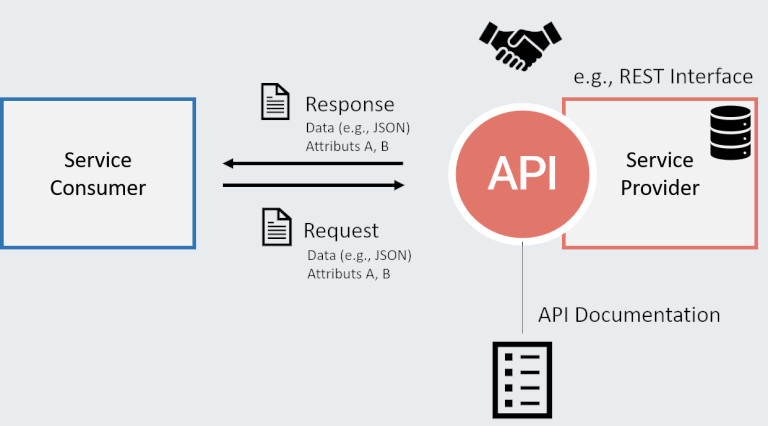
\includegraphics[width=\textwidth]{greg}
    \end{figure}
\end{frame}

\begin{frame}{Materials and Methods}
    \textbf{Storing data set}\\
    \vspace{2em}
    Since this is no trivial dataset with relations between game, teams, players and player stats storing it in CSV or other plain file format would be overkill. That's why SQL format was chosen, which allows:
    
    \begin{itemize}
        \item no need to write complex python code for parsing and choosing columns to data frame
        \item easy filtering of data by years, seasons or other categories
        \item updating data easy as a pie
    \end{itemize}
\end{frame}

\begin{frame}{Materials and Methods}
    \textbf{Storing data set}\\
    \vspace{2em}
   
    To be type agnostic another python framework was chosen to design and model database in easy to migrate manner. SQLAlchemy allows for shaping SQL database using python classes. Following schema was proposed:
\end{frame}

\begin{frame}{Materials and Methods}
    \begin{figure}[H]
        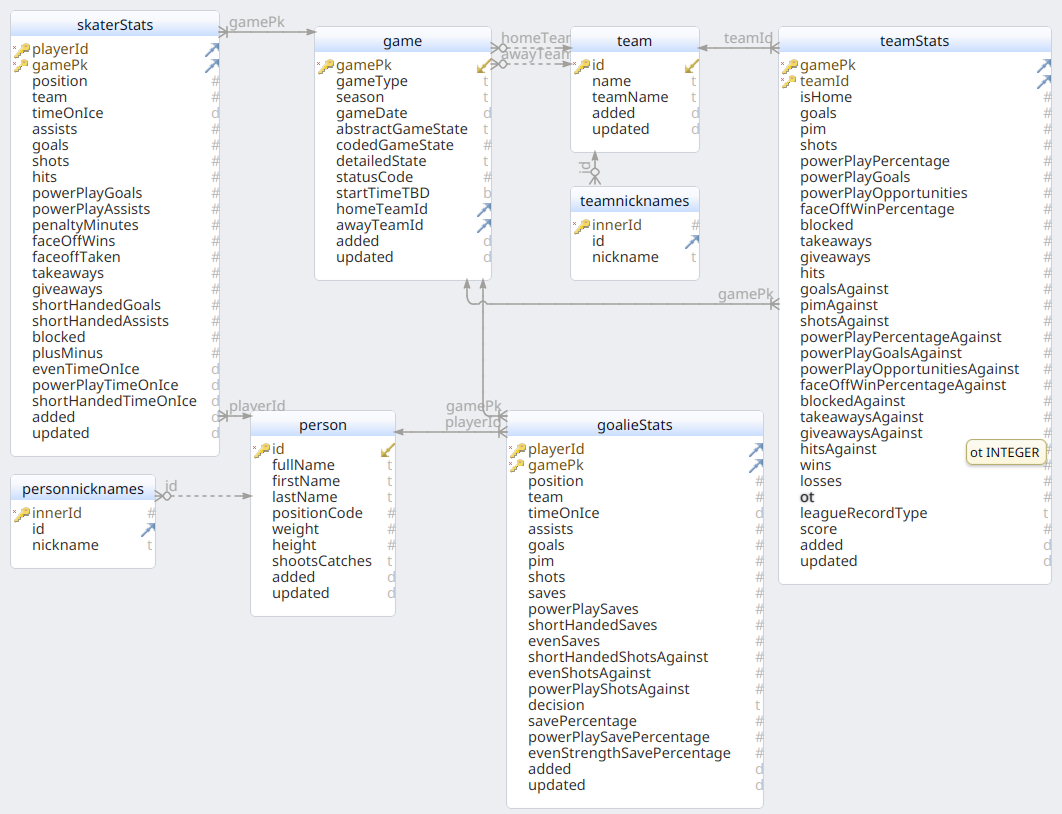
\includegraphics[height=0.9\textheight]{dbschema}
    \end{figure}
\end{frame}

\begin{frame}{Materials and Methods}
    \textbf{Shaping data frame}\\
    \vspace{2em}
    From person and skaterStats table following columns were chosen as candidates for data frame:\\
    \begin{minipage}[t]{0.45\textwidth}
        \begin{itemize}
            \item person.id
            \item person.positionCode
            \item person.weight,
            \item person.height,
            \item person.shootsCatches,
            \item skaterStats.timeOnIce,
            \item skaterStats.assists,
            \item skaterStats.goals,
            \item skaterStats.shots,
            \item skaterStats.hits,
            \item skaterStats.powerPlayGoals
            \item skaterStats.powerPlayAssists,
        \end{itemize}
    \end{minipage}
    \begin{minipage}[t]{0.45\textwidth}
        \begin{itemize}
            \item skaterStats.penaltyMinutes,
            \item skaterStats.faceOffWins,
            \item skaterStats.faceoffTaken,
            \item skaterStats.takeaways,
            \item skaterStats.giveaways,
            \item skaterStats.shortHandedGoals,
            \item skaterStats.shortHandedAssists,
            \item skaterStats.blocked,
            \item skaterStats.plusMinus,
            \item skaterStats.evenTimeOnIce,
            \item skaterStats.powerPlayTimeOnIce,
            \item skaterStats.shortHandedTimeOnIce
        \end{itemize}
    \end{minipage}
\end{frame} 

\begin{frame}{Materials and Methods}
    \textbf{Method of modeling}\\
    \vspace{2em}
    Scalable Vector Machine was used to o estimate the relationship between a dependent variable and independent variables with standard scaler as standardization of a dataset is a common requirement for many machine learning estimators: they might behave badly if the individual features do not more or less look like standard normally distributed data.
    
    \begin{figure}[H]
        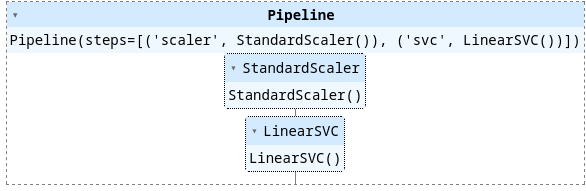
\includegraphics[width=\textwidth]{pipeline}
    \end{figure}
\end{frame}
